\section{PID-Regler \formelbuch{147}}

	\subsection{P-Regler - Stationärer Zustand \formelbuch{155}}
		Beim einfachsten linearen Regler, dem P-Typ, besteht ein proportionaler
		Zusammenhang zwischen Fehler $e$ und Stellgrösse $u$.\\
		Der P-Regler reagiert schnell, kann aber den Sprungfehler nicht vollständig
		eliminieren. Er hat einen stationären Fehler.
		
	
	\subsection{I-Regler \formelbuch{160}}
		Der reine I-Regler ist allgemein ungünstig, weil er relativ langsam arbeitet
		und die Stabilität schwacht. Ist aber die Regelstrecke nur erster Ordnung
		erziehlt man gute Ergebnisse mit dem I-Regler.\\
		Der I-Regler neigt zum Schwingen.\\
		Bei sprungförmigen Signalen, d.h. für Festwertregelungen hat der I-Regler
		keinen Fehler!
		
	
	\subsection{$PT_2$-Glied \formelbuch{163}}
		\begin{minipage}{5cm}
        \fbox{$T_\omega = 2T_m=\frac{2\pi}{\omega_n \sqrt{1-\zeta
        ^2}}=\frac{2\pi}{\omega}$}\\
        \fbox{$\omega = \frac{2\pi}{T_\omega}=2\pi f$}
        \end{minipage}
		\begin{minipage}{13cm}
        $T_\omega$: Schwingungsdauer\\
        $\omega_n$: Kennkreisfrequenz\\
        $\zeta$: \hspace{1.1mm} Dämpfungskonstante\\
        \end{minipage}\\
		\glqq Optimale Dämpfung\grqq\ bei $\Psi=45$ und $\zeta=\frac{1}{\sqrt{2}}$.
		Dabei erreicht die Regelgrösse $y$ nach $4.3\%$ Überschwingen rasch den
		Endwert.\\
		\begin{minipage}{7cm}
		$T^2\ddot{y}+2\zeta T \dot{y}+ y=Ku$\\
		$\ddot{y}+2\zeta\omega_n\dot{y}+\omega_n^2=\omega_n^2 Ku$
		\end{minipage}
		\begin{minipage}{11cm}
        $\ddot{y}+a_1\dot{y}+a_0 y=\ldots$\\
        $a_1=2\zeta\omega_n$\\
        $a_0=\omega_n^2$
        \end{minipage}
	
	\subsection{PI-Regler \formelbuch{174}}
		\begin{minipage}{15cm}
        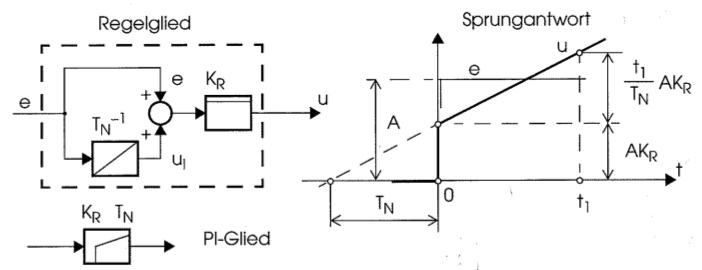
\includegraphics[angle={0},width=10cm]{./bilder/PI_Regler.jpg}
        \end{minipage}\\ \\
		\begin{minipage}{15cm}
        \fbox{$G(j\omega)=K_R \frac{1+j\omega T_N}{j\omega T_N}$}\qquad
        \fbox{$arg(G(j\omega))=\arctan(\omega T_N)-\frac{\pi}{2}$}
        \end{minipage}
		
	
	\subsection{D-Glied \formelbuch{179}}
		Der Differenzierer erzeugt eis Korrektursignal im voraus.\\
		Nachteilig ist, wenn die Regelgrösse verrauscht ist, dann werden die
		hochfrequenten Störsignale durch die Ableitung verstärkt.\\
		Ein LTI-System, welches ohne D-Glied darstellbar ist, gegebenenfalls durch
		Umformung des Blockdiagramms, heisst realisierbar.
	
	
	\subsection{PID-Regler \formelbuch{183} \formelbuch{383}}
	\fbox{$G(s) = K_R(1 + \frac{1}{j \omega T_N} + j \omega T_V )$}
	
	\subsection{PD-Regler \formelbuch{187} \formelbuch{383}}
	\fbox{$u=K_R at+K_R T_V a$} \qquad
	Das PD-Glied entspricht dem inversen PT$_1$-Glied.
	
	\subsection{Empirische Einstellregeln \formelbuch{188}}
		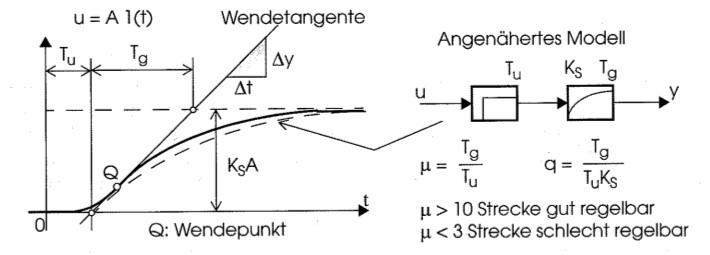
\includegraphics[width=13cm]{./bilder/Empirisch_Regeln.jpg}
		\begin{minipage}[b]{5cm}
        UTF des angenäherten Modells:\\ \\
		$G_0(j\omega)=\frac{K_s}{1+j\omega T_g}e^{-j\omega T_u}$
		\vspace{2.7cm}
		\end{minipage}\\
		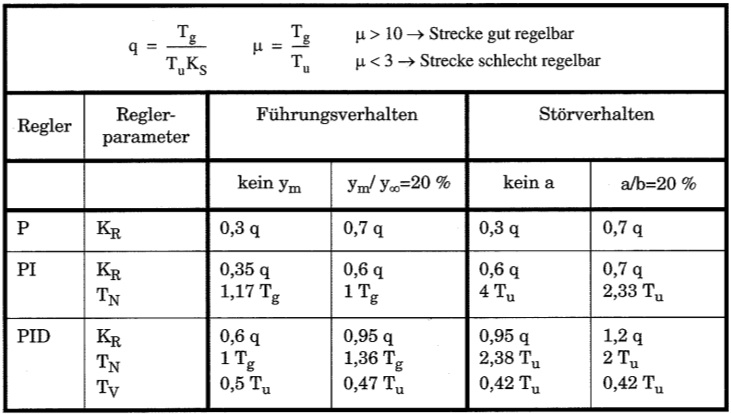
\includegraphics[width=13cm]{./bilder/CHR_Einst.jpg}
		\begin{minipage}[b]{5cm}
        $y_m$: \"Uberschwingen
        \vspace{4cm}
        \end{minipage}\\
		Reglereinstellung nach Chien-Hrones-Reswick\\
		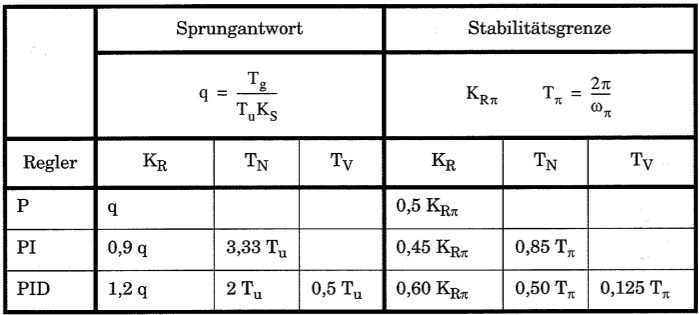
\includegraphics[width=13cm]{./bilder/ZN_Einst.jpg}\\
		Reglereinstellung nach Ziegler-Nichols
		
	\subsection{Wind-Up \formelbuch{200}}
		Die Folge eines \glqq wind-up-Phänomens\grqq\ ist einerseits ein konstanter
		Fehler und anderseits eine verzögert reagierende und damit stark überschwingende
		Regelgrösse.\\ \\
		\underline{wind-up entsteht durch:}\\
		\begin{itemize}
		\item bestehender Fehler
		\item I-Anteil im Regler
		\item Sättigung der Stellgrösse
		\end{itemize}
		
